\subsection{LZ78}

\begin{frame}{\FrameName}
	\begin{block}{LZ78}
		\begin{itemize}[<+->]
			\item Gänginger Kompressionsalgorithmus
			\item Abraham Lempel und Jacob Ziv (1978)
			\item Verwendung bei GIF und TIFF \PDFC{Erweiterung wird verwendet}
		\end{itemize}
	\end{block}
	\end{frame}

\begin{frame}{\FrameName}
\begin{block}{LZ78 - Datenstrukturen}
	\begin{itemize}[<+->]
		\item Strings als Sequenzen von Paaren $(i,c)$ dargestellt \linebreak \Hint{$i$...Index eines Vorgänger-Paares oder $0$$; c \in \Sigma$}
		\item Jedes Paar repräsentiert Substring
		\item Wenn $i$ gleich $0$ dann ist dieser Substring gleich $c$
		\item Andernfalls ist der Substring des $i$-ten Paares gefolgt von $c$
	\end{itemize}
\end{block}
\end{frame}

\begin{frame}{\FrameName}
\begin{block}{Beispiel}
	\Gap
	\Gap
	\begin{center}
		\only<1>{
			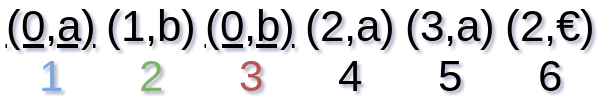
\includegraphics[width=0.8\textwidth]{Images/LZ78/blank}}
		\only<2>{
			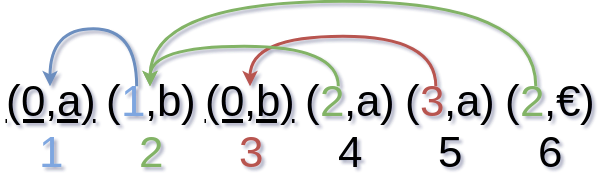
\includegraphics[width=0.8\textwidth]{Images/LZ78/withRefs}}
		\only<3>{
			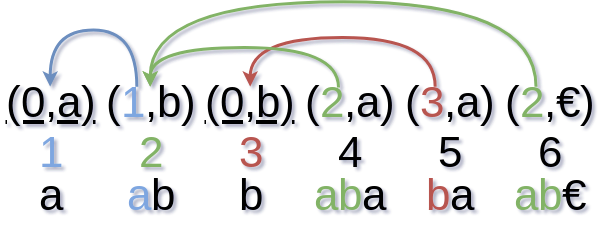
\includegraphics[width=0.8\textwidth]{Images/LZ78/full}}
	\end{center}
\end{block}
\end{frame}

\begin{frame}{\FrameName}
	\begin{block}{LZ78 Grammatiken}
		\begin{itemize}[<+->]
			\item Paar $\hat{=}$ Nichterminal
			\item $\begin{cases}
				X_j \rightarrow c, & i = 0\\
				X_j \rightarrow X_i c, & \text{sonst}
			\end{cases}$
			\item $S \rightarrow X_1 ... X_k$
			
		\end{itemize}
		\visible<4>{
			\begin{minipage}[t]{0.5\textwidth}
				$S \rightarrow \foreach \n in {1,2,3,4,5,6}{X_{\n}}$ 
				
	
				$X_1 \rightarrow a; X_2 \rightarrow X_1b;  X_3 \rightarrow b$
				$X_4 \rightarrow X_2a; X_5 \rightarrow X_3a; X_4 \rightarrow X_6\text{\euro}$
			\end{minipage}
			\begin{minipage}[c]{0.48\textwidth}
				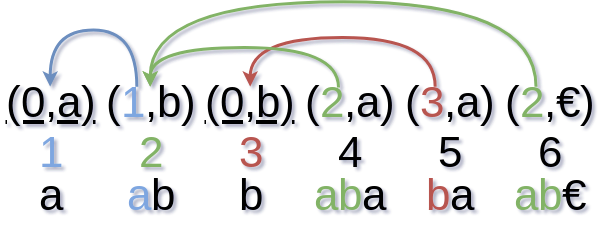
\includegraphics[width=\textwidth]{Images/LZ78/full}
			\end{minipage}
		}
	
	\end{block}
	\end{frame}

\begin{frame}{\FrameName}
\begin{block}{LZ78 - Algorithmus}
	\begin{itemize}[<+->]
		\item String wird Schrittweise in einem Durchlauf von links nach rechts in eine Sequenz von Paaren übersetzt
		\item Finde in jedem Schritt das kürzeste Präfix $\gamma$ des verbleibenden Strings das nicht Expansion eines bereits erzeugten Paars ist
		\item Am Ende des Strings muss eventuell ein weiteres Zeichen hinzugefügt werden
		\item Ein neues Paar wird an die Liste angehangen:
		\begin{enumerate}
			\item<4-> Wenn da $\gamma = 1$ ist füge $(0,\gamma)$ hinzu
			\item<5-> Andernfalls ist $\gamma = \alpha c$. \linebreak $\alpha$ ... Expansion eines Paars mit dem Index $i_\alpha$ \linebreak $\Rightarrow$ Paar: $(i,c)$
		\end{enumerate}
	\end{itemize}
\end{block}
\end{frame}

% Marking string sequence
\newcommand{\M}[1]{\textcolor{OrangeRed}{#1}}

\begin{frame}{\FrameName}
\begin{block}{Beispiel}
	\begin{description}[<+->]
		\item \M{a}abbababaab\euro
		\item $\underbrace{(0,a)}_{a}$ \M{ab}bababaab\euro
		\item $\underbrace{(0,a)}_{a}$ $\underbrace{(1,b)}_{ab}$ \M{b}ababaab\euro
		\item $\underbrace{(0,a)}_{a}$ $\underbrace{(1,b)}_{ab}$ $\underbrace{(0,b)}_{b}$ \M{aba}baab\euro
		\item $\underbrace{(0,a)}_{a}$ $\underbrace{(1,b)}_{ab}$ $\underbrace{(0,b)}_{b}$ $\underbrace{(2,a)}_{aba}$ \M{ba}ab\euro
		\item $\underbrace{(0,a)}_{a}$ $\underbrace{(1,b)}_{ab}$ $\underbrace{(0,b)}_{b}$ $\underbrace{(2,a)}_{aba}$ $\underbrace{(3,a)}_{ba}$ \M{ab\euro}
		\item $\underbrace{(0,a)}_{a}$ $\underbrace{(1,b)}_{ab}$ $\underbrace{(0,b)}_{b}$ $\underbrace{(2,a)}_{aba}$ $\underbrace{(3,a)}_{ba}$ $\underbrace{(2,\text{\euro})}_{ab\text{\euro}}$
	\end{description}
\end{block}
\end{frame}

\begin{frame}{\FrameName}
\begin{block}{LowerBound}
	\begin{center}
		\fbox{$ \alpha_k = a^{k(k+1)/2}(ba^k)^{(k+1)^2} $}
	\end{center}
	\begin{itemize}[<+->]
		\item $|\alpha_k | = k \frac{k+1}{2} + (1+k)(k+1)^2$ \linebreak
			$\phantom{|\alpha_k |} = k^3 + \frac{7}{2}k^2 + \frac{7}{2}k + 1$
		\item $ n = |\alpha_k | \in \Theta(k^3)$
	\end{itemize}
\end{block}
\end{frame}

\begin{frame}{\FrameName}
\begin{block}{UpperBound $m^*$}
	\begin{center}
		\fbox{$ \alpha_k = a^{k(k+1)/2}(ba^k)^{(k+1)^2} $}
	\end{center}
	\begin{itemize}[<+->]
		\item $m^* \in \mathcal{O}(1+ log(\frac{k^2+k}{2}) + log(k+1)^2 + 1+ log(k))$
		\item $m^* \in \mathcal{O}(log \thinspace k)$
		\item $m^* \in \mathcal{O}(log \thinspace n^\frac{1}{3}) = \mathcal{O}(log \thinspace n)$
	\end{itemize}
\end{block}
\end{frame}

\begin{frame}{\FrameName}
\begin{block}{LowerBound m}
	\begin{center}
		\fbox{$ \alpha_k = a^{k(k+1)/2}(ba^k)^{(k+1)^2} $}
	\end{center}
	\begin{itemize}[<+->]
		\item String wird in zwei Phasen in eine Paar-Sequenz übersetzt
		\item Erste Phase: alle Strings $a...a^k$ zu Paaren übersetzt
		\item Zweite Phase: $a^iba^j$ für alle $i,j \in [0,k]$ wird ein Paar erstellt
		\item $m \in \Omega(\sum_{z=1}^k z + (k+1)^2) = \Omega(k^2)$
		\item $m \in \Omega(n^{2/3})$
	\end{itemize}
\end{block}
\end{frame}

\begin{frame}{\FrameName}
\begin{block}{LowerBound}
	\begin{center}
		\fbox{$ \alpha_k = a^{k(k+1)/2}(ba^k)^{(k+1)^2} $}
	\end{center}
	\begin{itemize}[<+->]
		\item $m^* \in \mathcal{O}(log \thinspace n)$
		\item $m \in \Omega(n^{2/3})$
		\item $a(n) \in \Omega(\frac{n^{2/3}}{log \thinspace n})$
	\end{itemize}
\end{block}
\end{frame}

\begin{frame}{\FrameName}
	\begin{block}{Upper bound}
		\visible<1->{
			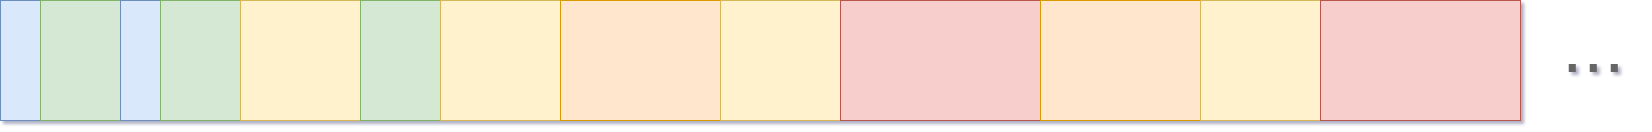
\includegraphics[width=0.98\textwidth]{Images/LZ78/ub_blank}}
			\Gap
		\visible<2->{
			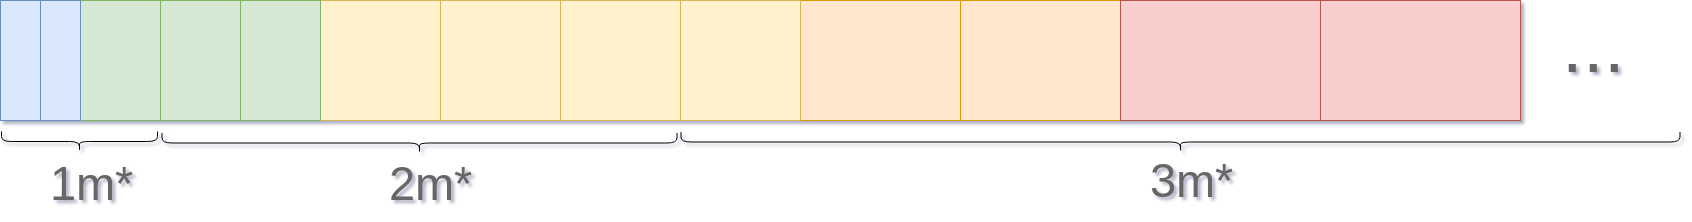
\includegraphics[width=0.98\textwidth]{Images/LZ78/ub_sort}}
			\Gap
		\visible<3->{
			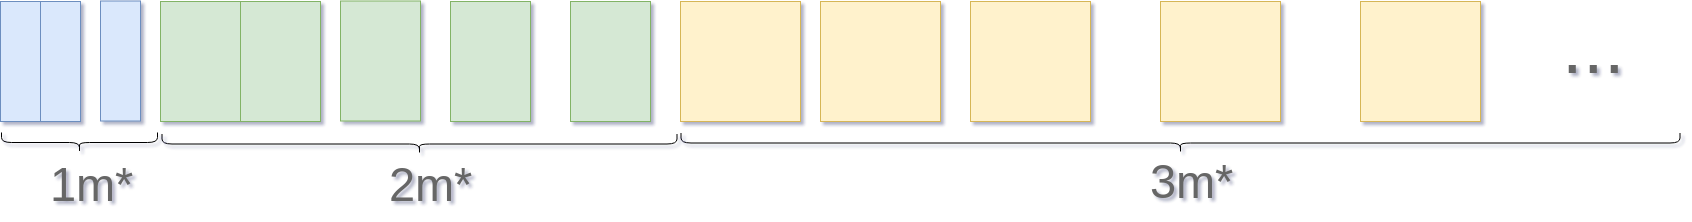
\includegraphics[width=0.98\textwidth]{Images/LZ78/ub_underestimate}}
	\end{block}
	\end{frame}

	\begin{frame}{\FrameName}
		\begin{block}{Upper bound}
			\visible<1->{
				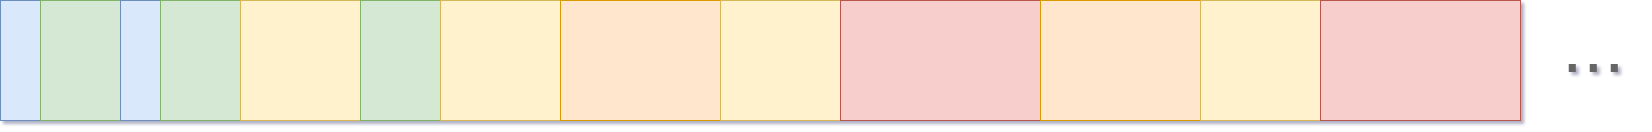
\includegraphics[width=0.98\textwidth]{Images/LZ78/ub_blank}}
				\Gap
			\visible<2->{
				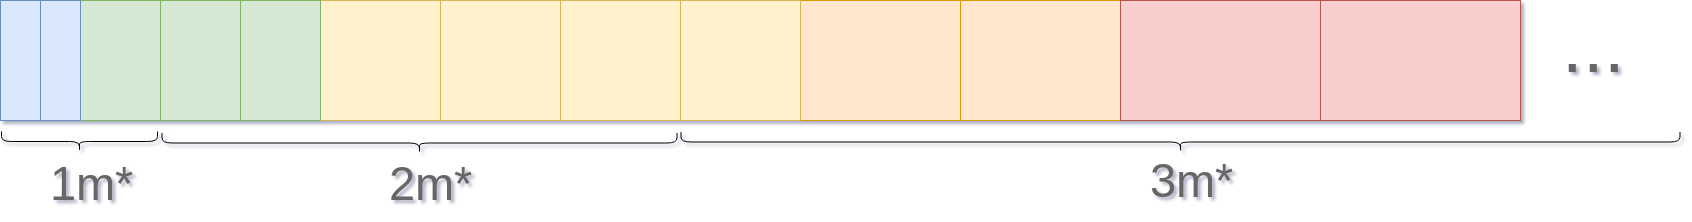
\includegraphics[width=0.98\textwidth]{Images/LZ78/ub_sort}}
				\Gap
			\visible<3->{
				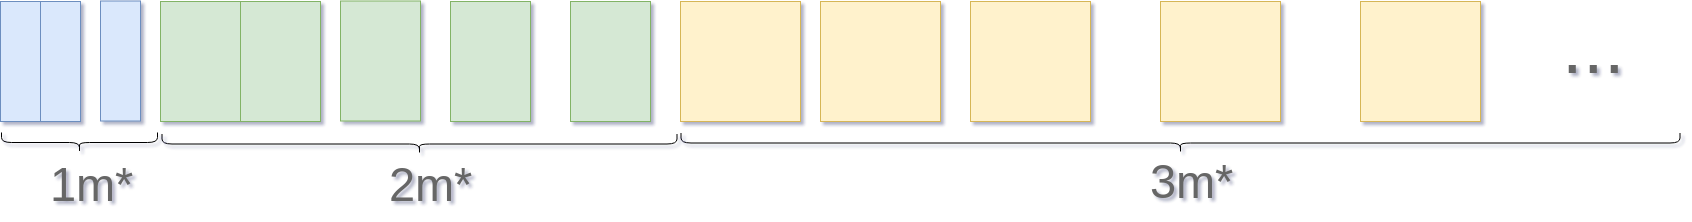
\includegraphics[width=0.98\textwidth]{Images/LZ78/ub_underestimate}}
		\end{block}
		\end{frame}